\chapter{Diagramma delle velocità}

Per creare il diagramma delle velocità si usa il comando Geometry/italian checks/speed diagram impostando la normativa italiana e la tipologia di strada, F extraurbana nel nostro caso, e la velocita massima di progetto. Successivamente basterà cliccare sulla sopraelevazione per ottenere il diagramma \ref{Diagramma delle velocità}.

\begin{figure}[H]
    \includegraphics[width=\textwidth]{Figures/Diagramma delle velocità.png}
      \caption{Diagramma delle velocità}
      \label{Diagramma delle velocità}
\end{figure}

Ottenuto il diagramma delle velocità e il profilo dei cigli si può procedere con la verifica  dei criteri di Normativa utilizzando il comando Geometry/Italian checks/orizontal vertical checks.

\begin{figure}[H]
    \includegraphics[width=\textwidth]{Figures/Controllo delle velocità.png}
      \caption{Controllo delle velocità}
      \label{Controllo delle velocità}
\end{figure}

\begin{figure}[H]
    \centering
    \begin{minipage}[b]{0.45\textwidth}
      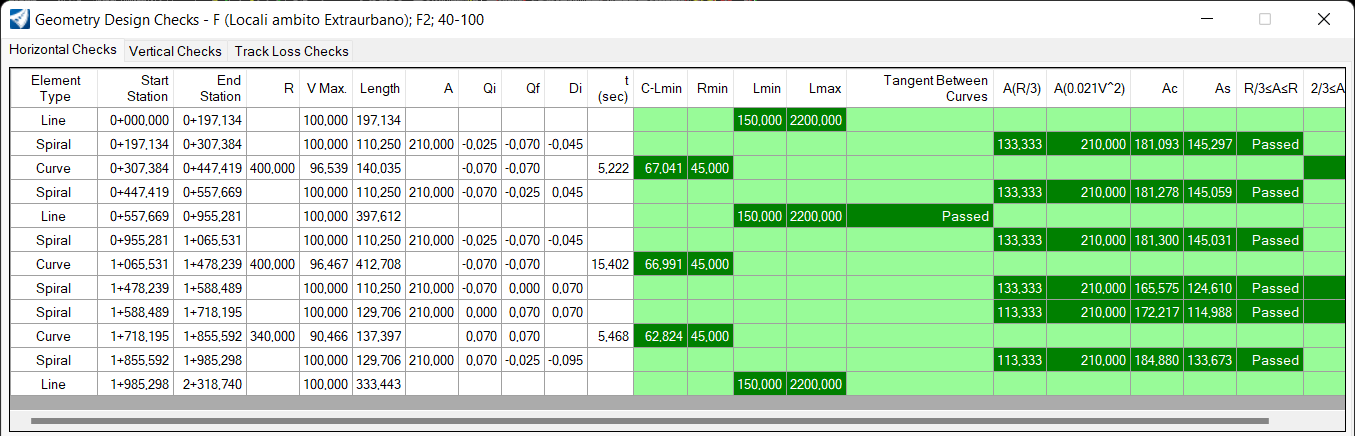
\includegraphics[width=\textwidth]{Figures/Controllo planimetrico.png}
      \caption{Controllo planimetrico}
      \label{Controllo planimetrico}
    \end{minipage}
    \hfill
    \begin{minipage}[b]{0.45\textwidth}
      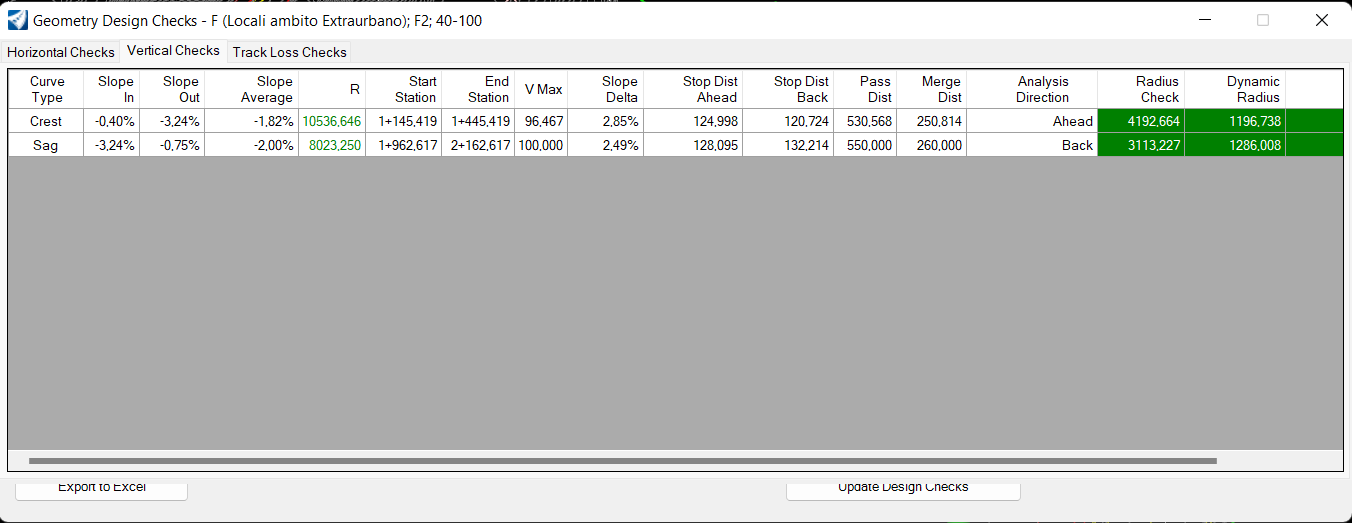
\includegraphics[width=\textwidth]{Figures/Controllo altimetrico.png}
      \caption{Controllo altimetrico}
      \label{Controllo altimetrico}
    \end{minipage}
  \end{figure}

  \begin{figure}[H]
    \centering
    \begin{minipage}[b]{0.45\textwidth}
      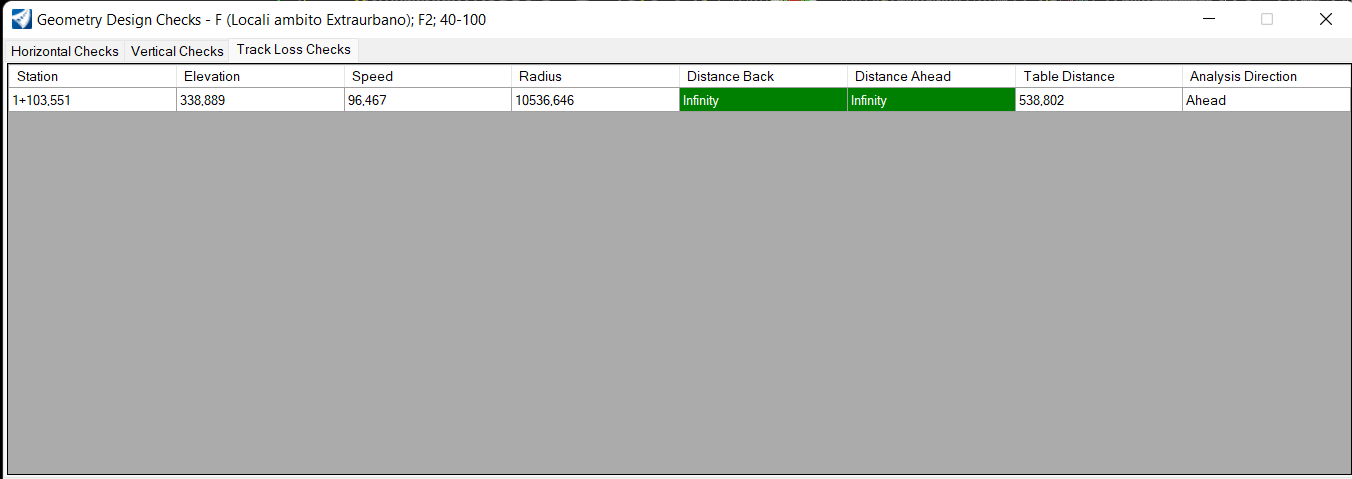
\includegraphics[width=\textwidth]{Figures/Perdita di tracciato.png}
      \caption{Perdita di tracciato}
      \label{Perdita di tracciato}
    \end{minipage}
    \hfill
    \begin{minipage}[b]{0.45\textwidth}
      \includegraphics[width=\textwidth]{Figures/Visibilità.png}
      \caption{Visibilità}
      \label{Visibilità}
    \end{minipage}
  \end{figure}